\begin{figure}[H]
    \centering
    \begin{adjustbox}{width=3cm,margin=11cm -12cm}
      
\includegraphics[width=12cm]{src/delay/delay-low.png}%
    \end{adjustbox}
    \begin{adjustbox}{width=10.5cm,center}
      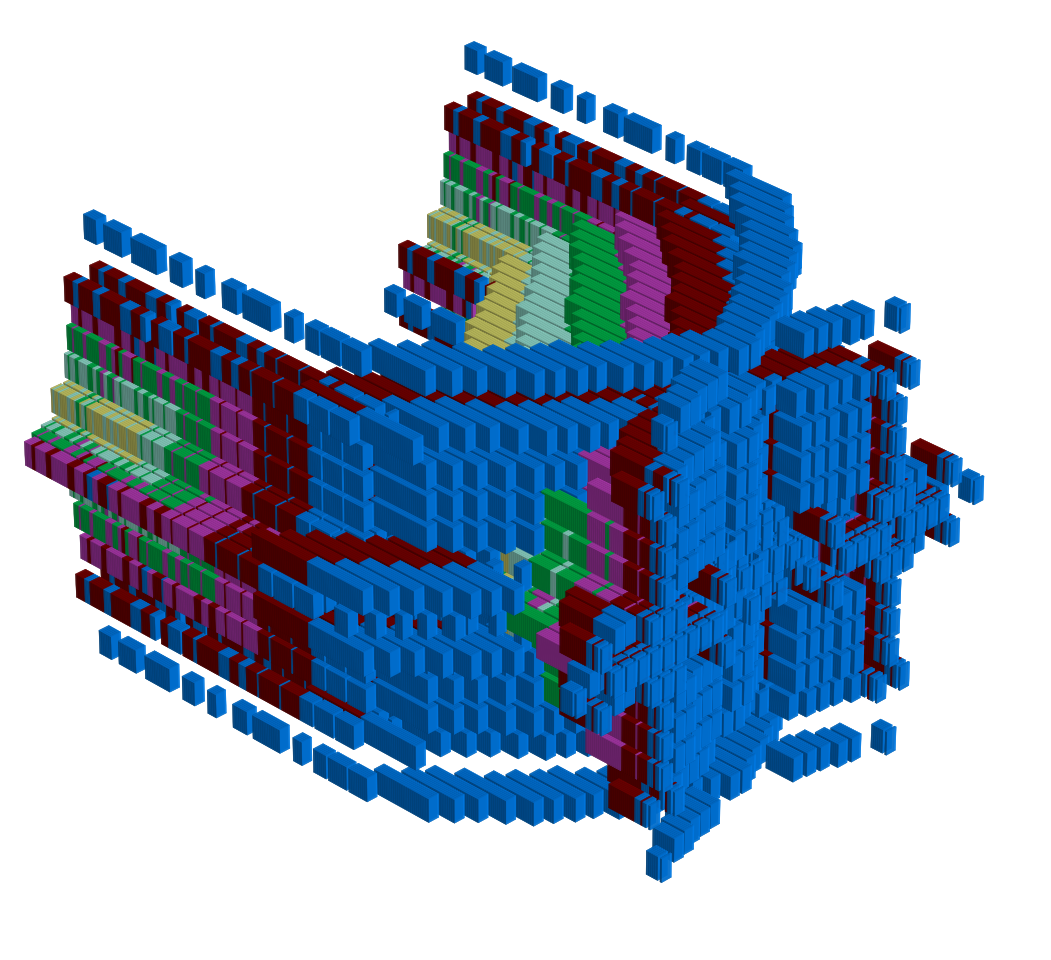
\includegraphics[width=12cm]{src/delay/pattern0-45.png}%
    \end{adjustbox}
    \begin{adjustbox}{width=3cm,margin=11cm -12cm}
      
\includegraphics[width=12cm]{src/delay/delay-high.png}%
    \end{adjustbox}
    \begin{adjustbox}{width=10.5cm,margin=0cm -2cm}
      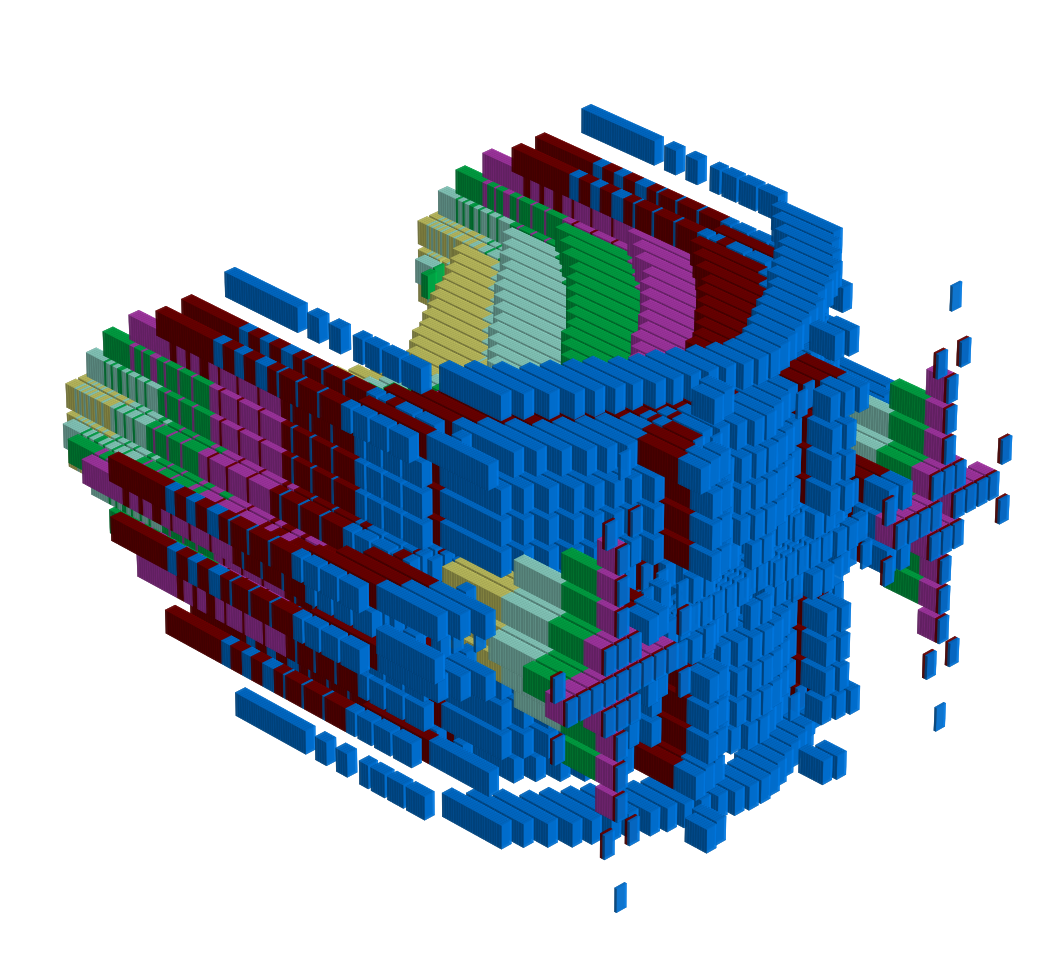
\includegraphics[width=12cm]{src/delay/pattern1-45.png}%
    \end{adjustbox}
    \caption{Effect of low and high values for Smoothing Delay}
\end{figure}
\clearpage

\section*{tentative tracking} 
\label{sec:tracking}
\lstset{style=6502Style}
\lstset{ 
   aboveskip=5pt,
   belowskip=0pt,
}

\begin{definition}[Jeffrey Says]
\setlength{\intextsep}{0pt}%
\setlength{\columnsep}{3pt}%
\begin{wrapfigure}{l}{0.12\textwidth}

\includegraphics[width=\linewidth]{src/callout/psych.png} 
\end{wrapfigure}
\small
\textbf{T to Activate:} Controls whether logic-seeking is used in
the buffer or not. The upshot of this for you is a slightly different
feel - continuous but fragmented when ON, or together-ish bursts
when OFF. Try it.
\\
\end{definition}

\clearpage
\textbf{Lines 1189-1231. \icode{\textbf{CheckKeyboardInput}}} 
\begin{lstlisting}
;-------------------------------------------------------
; CheckKeyboardInput
;-------------------------------------------------------
CheckKeyboardInput   
    ...
MaybeTPressed   
    CMP #KEY_T ; T pressed.
    BNE CheckIfPresetKeysPressed

    ;"T: Controls whether logic-seeking is used in the buffer or not. The upshot of 
    ; this for you is a slightly different feel - continuous but fragmented when ON,
    ; or together-ish bursts when OFF. "
    LDA trackingActivated
    EOR #$FF
    STA trackingActivated
    AND #$01
    ASL 
    ASL 
    ASL 
    ASL 
    TAY 
    JSR ClearLastLineOfScreen

    LDX #$00
txtTrackingLoop   
    LDA txtTrackingOnOff,Y
    STA lastLineBufferPtr,X
    INY 
    INX 
    CPX #$10
    BNE txtTrackingLoop

    JMP WriteLastLineBufferToScreen
    RTS 
\end{lstlisting}
\clearpage

\textbf{Lines 1189-1231. \icode{\textbf{CheckKeyboardInput}}:} 
\clearpage
\clearpage
\textbf{Lines 1189-1231. \icode{\textbf{MainInterruptHandler}}} 
\begin{lstlisting}
;-------------------------------------------------------
; MainInterruptHandler
; By default this runs every 1/60th of a second. 
; Its main job is to fill the pixel buffers (e.g.
; pixelXPositionArray, pixelYPositionArray and so on)
; so that the MainPaintLoop can use them to paint the
; screen. The counter countStepsBeforeCheckingJoystickInput
; ensures that we only update the pixel buffers every 256th
; time the interrupt is called. stepsRemainingInSequencerSequence
; does the same for the sequencer. 
;-------------------------------------------------------
MainInterruptHandler
        ...
        ; Finally, update the pixel buffers with a byte
        ; each for the current pattern.        
UpdatePixelBuffersForPattern    
        INC currentStepCount
        LDA currentStepCount
        CMP bufferLength
        BNE UpdateBaseLevelArray

        LDA #$00
        STA currentStepCount

UpdateBaseLevelArray   
        TAX 
        LDA currentColorIndexArray,X
        CMP #$FF
        BEQ UpdatePositionArrays

CheckIfTrackingActivated
        LDA previousIndexToPixelBuffers
        AND trackingActivated
        BEQ DrawCursorAndReturnFromInterrupt
        TAX 
        LDA currentColorIndexArray,X
        CMP #$FF
        BNE DrawCursorAndReturnFromInterrupt

        STX currentStepCount

UpdatePositionArrays   
        LDA cursorXPosition
        STA pixelXPositionArray,X
        LDA cursorYPosition
        STA pixelYPositionArray,X

\end{lstlisting}
\clearpage

\textbf{Lines 1189-1231. \icode{\textbf{CheckIfTrackingActivated}}:} 
\clearpage
